%-< SECTION >--------------------------------------------------------------------
\section{Simulation Model}\label{sec:sim_model}

% -< SUB SECTION
% >--------------------------------------------------------------------
% \subsection{Description of ns-3}\label{subsec:descriptionns-3}
ns-3~\cite{ns3} is a popular and free discrete-event network simulator for networking research. % To be closer to the real implementation (in a real Operating System), easily include C-based implementation codes, ease debugging and reduce the cost on maintaining in a long term, C++ is prioritized to be the unique programming language for ns-3 \ed{BD: I personally don't think C++ is easy to debug\ldots  Is it really important to explain why C++ is used for coding in ns-3?  I'm not sure}. 
Besides, ns-3 offers the possibility to visualize the simulation instance so to allow the users to visually confirm the packets flow as they expect. Thus, we choose ns-3 to develop our LISP/LISP-MN simulator.


% -< SUB SECTION
% >--------------------------------------------------------------------
\subsection{Modifications to ns-3}
\label{subsec:modifyns-3}
% -< FIGURE
% >--------------------------------------------------------------------
\begin{figure*}[!t] \centering
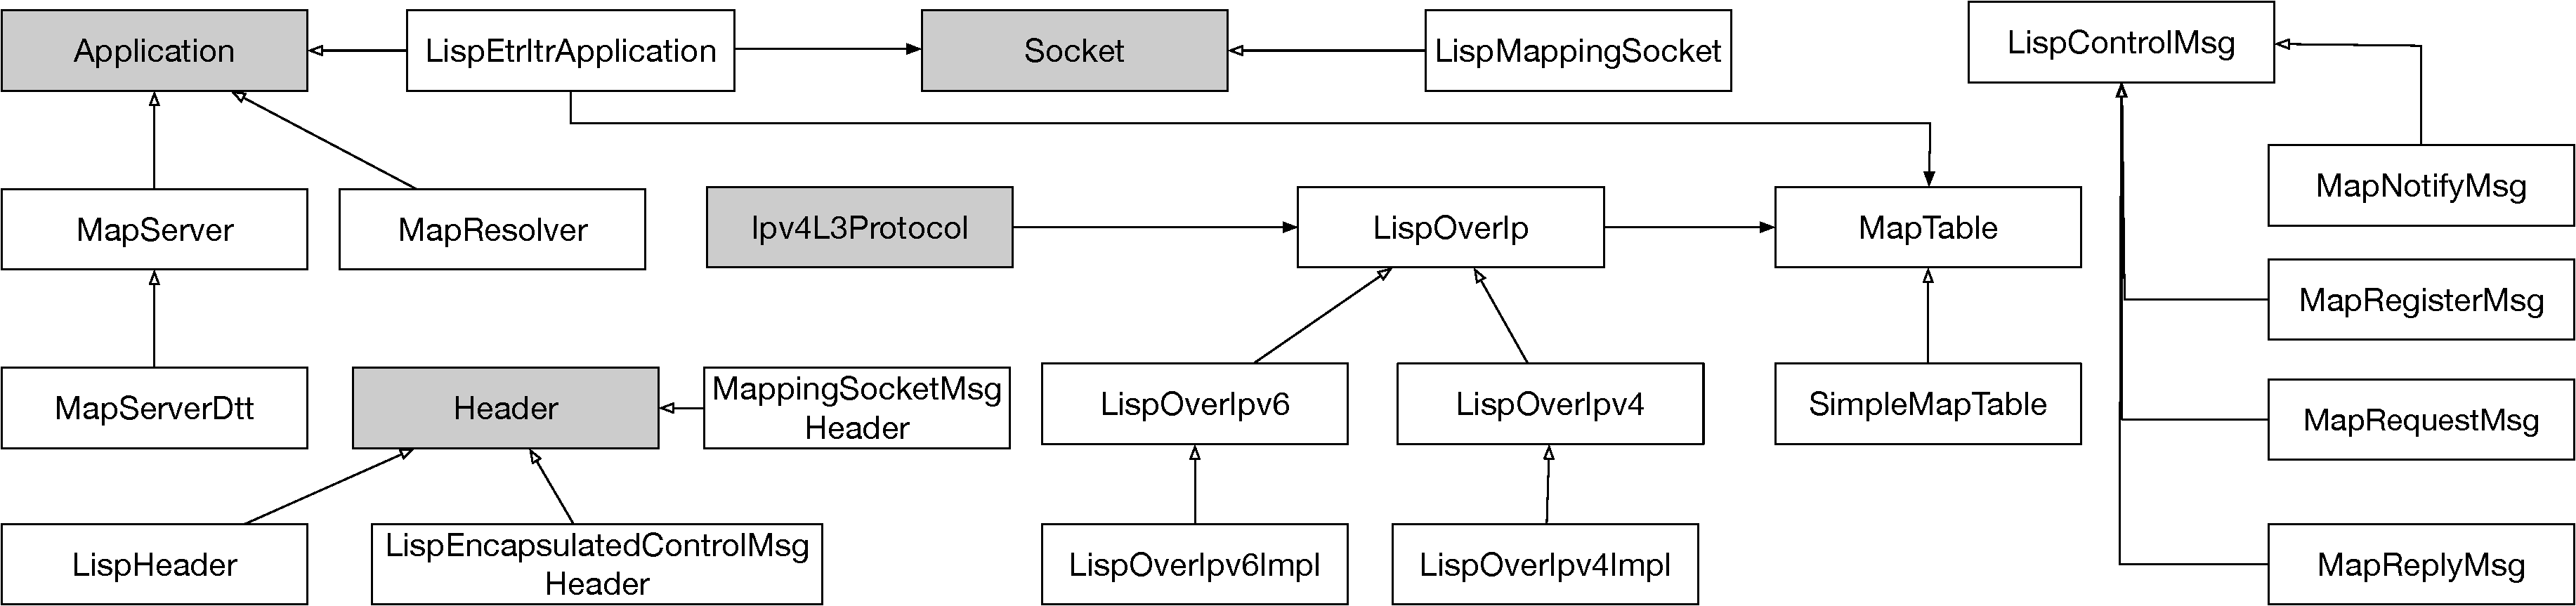
\includegraphics[width=\textwidth]{Pics/LISP-NS3-UML} \caption{UML diagram of
LISP/LISP-MN implementation. The solid arrow refers to a composition relation,
while the blank one refers to a inheritance relation.}
	\label{LISP-UML}
\end{figure*}
% -< END FIGURE
% >--------------------------------------------------------------------
Our implementation \ed{BD: should be open source.  Remind here the URL towards
the repo} is under ns-3.26 and based on LISP~\cite{ietf-lisp-rfc6830bis-03} and
LISP-MN standards~\cite{meyer-lisp-mn-16}. The main classes are shown in
Fig.~\ref{LISP-UML} in form of UML diagram. The blank blocks refer to the
classes that we added into ns-3, while darker blocks are classes already in
ns-3. As a design choice, we implement LISP/LISP-MN functionalities by modifying
and extending the \emph{internet} module of ns-3, instead of creating a new
independent module. The justification of this design is that LISP/LISP-MN and
legacy internet module have an interdependent relationship. However, this kind
of mutually dependent relationship between modules is not supported by ns-3.
Inspired by the OpenLISP design~\cite{saucez2009openlisp}, the Data Plane
implementation is in ``kernel space'' (i.e., ns-3 \emph{TCP/IP stack}) and the
Control Plane is implemented in ``user space'' (i.e., ns-3 \emph{Application}). 
The communication between LISP Data and Control Plane is ensured through a
dedicated socket (i.e., \emph{LispMappingSocket}) that inherits from the ns-3
\emph{Socket} class. It should be noted that our implementation only supports
IPv4 at time of  writing. The IPv6 support 
% (i.e. the implementation related to IPv6 such as \emph{LispOverIpv6Impl}) 
is still under construction.


% -< SUBSUB SECTION
% >--------------------------------------------------------------------
\subsubsection{Implementation of LISP Data Plane}\label{subsec:modifyInternet}
A LISP-compatible node (terminal or router) should be capable of determining
whether a packet should be passed to LISP-related procedure and retrieving the
associated mapping information if necessary. To this end, a new class called
\emph{LispOverIp} and its extended classes (refer to Fig.~\ref{LISP-UML}) are
added to ns-3 \emph{internet} module. This class is in charge of checking
whether necessary LISP-related operations (\texttt{NeedEncapsulation()},
\texttt{NeedDecapsulation()}) must be done, and of encapsulating conventional IP
packets (i.e., \texttt{LispOutput()}) as well as decapsulating LISP
packets(\texttt{LispInput()}). It also contains a smart pointer to the
LISP database and LISP cache.
Both data structures (store the EID-RLOC mapping information) are represented by
the class \emph{SimpleMapTable} that inherits from \emph{MapTable}. The
inheritance mechanism allows other users to implement their own implementation
of LISP database and cache. To support LISP functionalities, the \emph{Ipv4L3Protcol},
which is the IP layer implementation in ns-3, contains one \emph{LispOverIp}
object and \emph{Ipv4L3Protcol}'s packet transmission and reception procedures
are accordingly adapted.

To process outgoing packets, the adapted \texttt{send()} in \emph{Ipv4L3Protcol}
first verifies whether the \emph{LispOverIp} object is present. If yes, some
checks are then conducted to determine that this packet should be processed by
\texttt{LispOutput()} (to encapsulate the packets) or by conventional packet
transmission routine. For example, if both source and destination IP addresses
of this packet belong to the same network, the LISP-related process (e.g.,
encapsulation) is skipped and this packet is processed as in a non-LISP network.
Otherwise, EID-RLOC mapping information is searched from LISP cache and LISP
database on LISP-MN node. In case of a cache miss, the packet is dropped and
\texttt{SendNotifyMessage()} in \emph{LispOverIp} notifies, via a
\emph{LispMappingSocket} socket, the \emph{LispEtrItrApplication} that runs on
LISP-MN node. At the reception of the cache miss event from LISP Data Plane
(i.e., \emph{LispOverIp} object), \emph{LispEtrItrApplication} initiates a
Map-Request message to LISP mapping system. At the reception of the Map-Reply,
the received EID-RLOC mapping is inserted into LISP cache. It should be noted
that as an implementation choice, before the reception of Map-Reply message, all
transmitted packets with the required RLOC as destination are dropped. One can
also design a buffer to queue these packets and resend them once the required
mapping information is received via Map-Reply.
The advantage of such an implementation is to reduce the packet loss rate.

For an incoming packet, if the destination of this packet is the node itself,
the packet is processed by \texttt{LocalDelivery()} in \emph{Ipv4L3Protocol}.
Before passing to transport layer, \texttt{LocalDelivery()} checks if the packet
should be decapsulated. If yes, it is passed to \texttt{LispInput()}, in
which the packet is decapsulated and reinjected in the IP stack. If the received
packet destination is not this node, the packet is processed by patched
\texttt{IpForward()} method. This packet may be ended up with LISP encapsulation
procedure.


\subsubsection{Implementation of LISP Control Plane}\label{subsec:control-plane-impl}
The implementation of LISP Control Plane at least should provide ITR/ETR, MR,
and MS. In practice, ETR and ITR functionalities are usually placed on a same
router. In our implementation, they are included in the
\emph{LispEtrItrApplication} class. A ns-3 node that runs
\emph{LispEtrItrApplication} is a LISP-compatible router. It should be able to
communicate with \emph{LispOverIp} on the same node (e.g., inform about cache
miss) and other LISP-compatible routers (e.g., Map-Request/Map-Reply). To
support LISP-MN feature, \emph{LispEtrItrApplication} also communicates with
DHCP client application. For example, once a LISP-MN obtains an IP address from
the DHCP server, \emph{LispEtrItrApplication} receives the corresponding
EID-RLOC mapping and sends a Map-Register message~\cite{meyer-lisp-mn-16}.

A node that runs a \emph{MapServer} application is the MS in a LISP-supported
network. This class maintains a LISP database to store the EID-RLOC mapping
information, learned from Map-Register message at the initialization stage. In
current implementation, the role of MR is to receive the Map-Request message
from xTR and forward it to the MS.

% -< SUBSUB SECTION
% >--------------------------------------------------------------------
\subsubsection{Integration of TUN net interface card}\label{subsec:tundevice}
To support mobility, LISP-MN actually can be regarded as a small LISP-Site, in
which xTR functionalities and DHCP service are implemented, as well as
configured address of MR and MS. As a LISP-MN node, it has a static permanent
EID and dynamic RLOC assigned by the DHCP server. To differentiate with
conventional RLOC of xTR interface, such kind of RLOC is referred to as the
local RLOC (LRLOC). Different from conventional LISP node, at least two net
interface cards (NIC) are installed into LISP-MN. One is \emph{WifiNetDevice},
the other is a TUN type card. The DHCP client application runs on LISP-MN's
\emph{WifiNetDevice} and thus the LRLOC is allocated to this card. The permanent
EID is assigned to \emph{VirtualNetDevice} net card. We modify the node's
routing table so that each packet's inner header contains IP address on
\emph{TunNetDevice} and outer header contains IP address of \emph{WifiNetDevice}
as source address.

% -< SUBSUB SECTION
% >--------------------------------------------------------------------
\subsubsection{Integration of DHCP}\label{subsec:DHCP}
To support mobility within conventional LISP node, a modified DHCP client
application is integrated into ns-3 node. To be compatible with LISP
functionality, DHCP client application is modified. Once the DHCP client
receives an allocated IP address (i.e., LRLOC), it notifies the
\emph{LispEtrItrApplication} (i.e., LISP Control Plane) by sending a dedicated
message that contains the EID-LRLOC mapping. \emph{LispEtrItrApplication} is in
charge of populating the received mapping entry into LISP database. During the
mobility process, when wireless link is down, the DHCP client flushes the
LISP-MN database and populates the database again at the reception of a new
LRLOC.
